\section{Introdução} % Seções são adicionadas para organizar sua apresentação em blocos discretos, todas as seções e subseções são automaticamente exibidas no índice como uma visão geral da apresentação, mas NÃO são exibidas como slides separados.

%----------------------------------------------------------------------------------------

% \begin{frame}
% 	\frametitle{Problema}
% 	\begin{itemize}[<+(1)->]
% 		\item Avaliar o desempenho de modelos na resolução de Open-Ended Tasks é difícil.
% 		\item Novas métricas automatizadas seguem sendo desenvolvidas.
% 		\item Qual a melhor métrica para cada situação?
% 		\only<5>{
% 			\item Como as métricas se correlacionam com avaliações humanas?
% 		}
% 		\only<6>{
% 			\item \textbf{Como as métricas se correlacionam com avaliações humanas?}
% 		}
% 	\end{itemize}
% \end{frame}

%----------------------------------------------------------------------------------------

% \begin{frame}
% 	\frametitle{Objetivo}
% 	Mensurar a correlação entre diferentes métricas de avaliação automatizadas e 
% 	a forma de avaliação humana no âmbito de open-ended tasks em português.
% \end{frame}

%----------------------------------------------------------------------------------------

% \begin{frame}
% 	\only<1>{
% 		\frametitle{Processamento de Linguagem Natural}
% 	}
% 	\only<2>{
% 		\frametitle{Processamento de Linguagem Natural (PLN)}
% 	}
% 	\only<3->{
% 		\frametitle{PLN}
% 	}
% 	\only<3-8>{
% 		\begin{columns}
% 			\column{0.5\linewidth}
% 				Permitir ao modelo:
% 				\begin{itemize}[<+(3)-8>]
% 					\item Compreender
% 					\item Interpretar
% 					\item Analisar
% 					\item Reproduzir
% 				\end{itemize}
% 			\column{0.5\linewidth}
% 				\only<8>{
% 					\begin{figure}
% 						
\includegraphics[width=\textwidth]{linguagem-natural.jpg}
% 						\caption{Linguagem Natural}
% 					\end{figure}
% 				}
% 		\end{columns}
% 	}
% 	\only<9>{
% 		\begin{figure}
% 			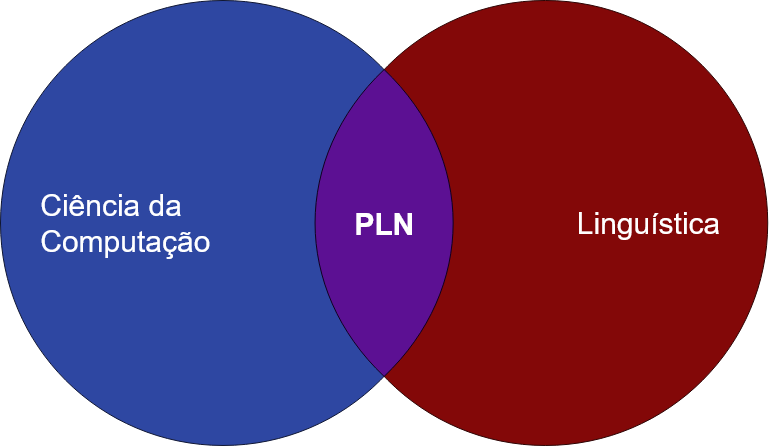
\includegraphics[width=0.8\textwidth]{PLN-AREA.png}
% 		\end{figure}
% 	}
% 	\only<10>{
% 		\begin{figure}
% 			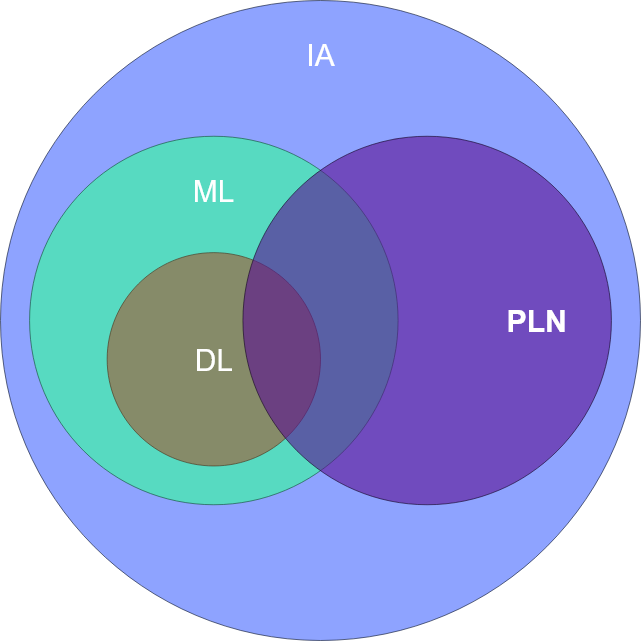
\includegraphics[height=0.8\textheight]{PLN-IA.png}
% 		\end{figure}
% 	}
% 	\only<11>{
% 		Desde a concepção dos primeiros computadores, já se sonhava com a ideia 
% 		de que os mesmos conseguissem compreender a linguagem humana.
% 	}
% \end{frame}

% %----------------------------------------------------------------------------------------

% \begin{frame}
% 	\only<1-4>{
% 		\frametitle{Teste de Turing}
% 	}
% 	\only<5->{
% 		\frametitle{Problemas do Teste}
% 	}
% 	\only<1-3>{
% 		\begin{columns}
% 			\column{0.5\linewidth}
% 				\begin{itemize}[<+(1)-3>]
% 					\item Proposto em 1950.
% 					\item \textbf{Máquina} consegue emular comportamento \textbf{humano}.
% 				\end{itemize}
% 			\column{0.5\linewidth}
% 				\begin{figure}
% 					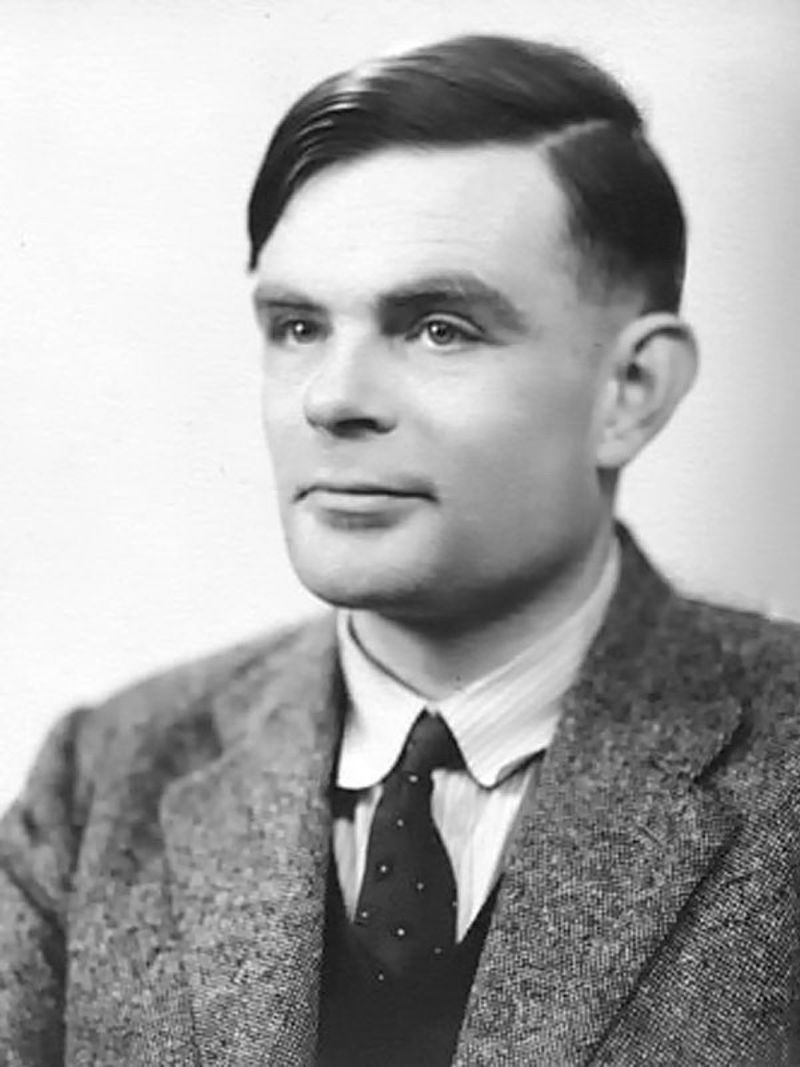
\includegraphics[height=0.6\textheight]{Turing.jpg}
% 					\caption{Alan Turing}
% 				\end{figure}
% 		\end{columns}
% 	}
% 	\only<4>{
% 		\begin{figure}
% 			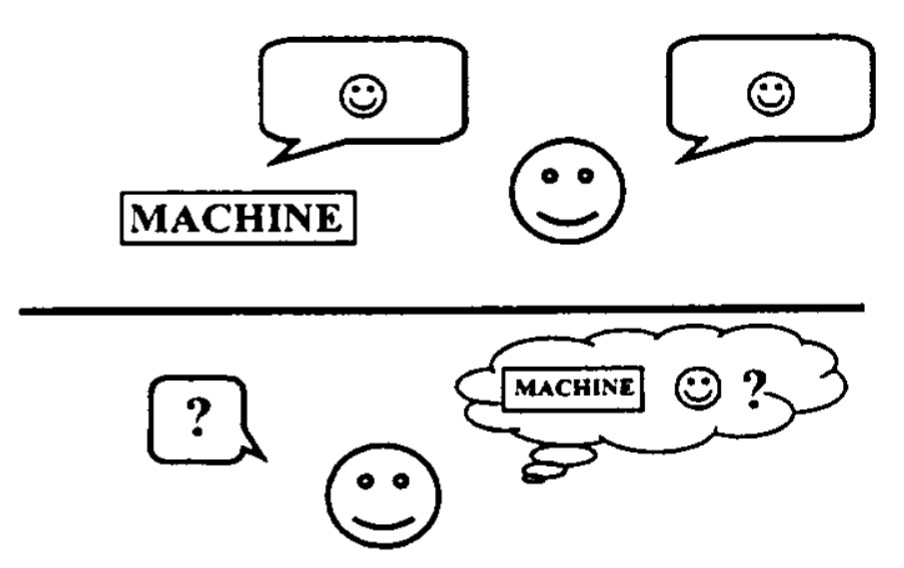
\includegraphics[width=0.8\textwidth]{Turing Test.jpg}
% 			% \caption{Fonte: \citet{pinar2000turing}.}
% 		\end{figure}
% 	}
% 	\only<5->{
% 		\begin{itemize}[<+(5)->]
% 			\item Fácil Manipulação.
% 			\item Falta de Autoconsciência.
% 			\only<8>{
% 				\item Imitação vs Compreensão.
% 			}
% 			\only<9>{
% 				\item \textbf{Imitação vs Compreensão.}
% 			}
% 		\end{itemize}
% 	}
% \end{frame}

% %----------------------------------------------------------------------------------------

% \begin{frame}
% 	\frametitle{Argumento do Quarto Chinês}
% 	\only<1-3>{
% 		\begin{columns}
% 			\column{0.5\linewidth}
% 				\begin{itemize}[<+(1)-3>]
% 					\item Proposto em 1980.
% 					\item Questiona pressuposições do Teste de Turing.
% 				\end{itemize}
% 			\column{0.5\linewidth}
% 				\begin{figure}
% 					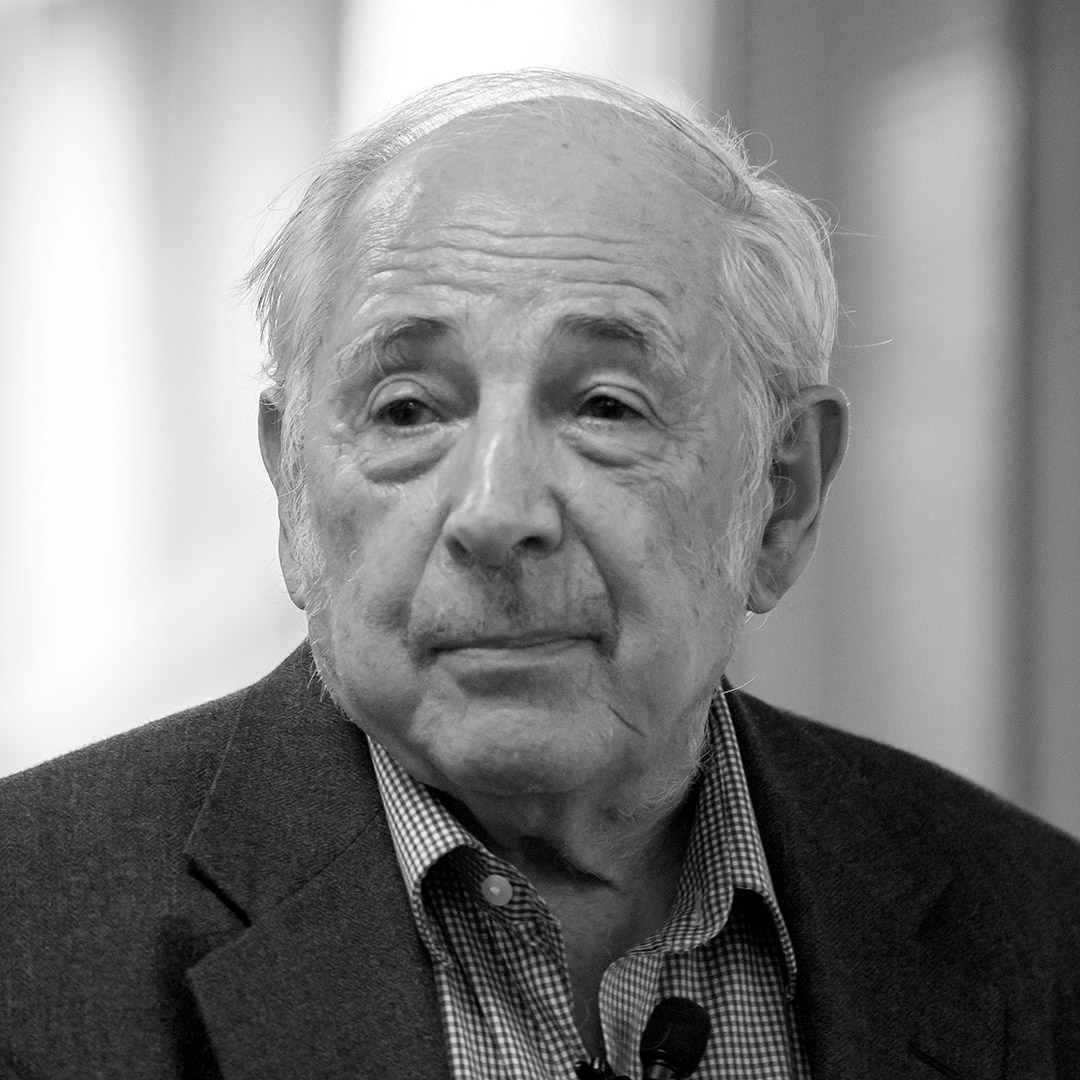
\includegraphics[height=0.6\textheight]{John_Searle.jpg}
% 					\caption{John R. Searle}
% 				\end{figure}
% 		\end{columns}
% 	}
% 	\only<4>{
% 		\begin{figure}
% 			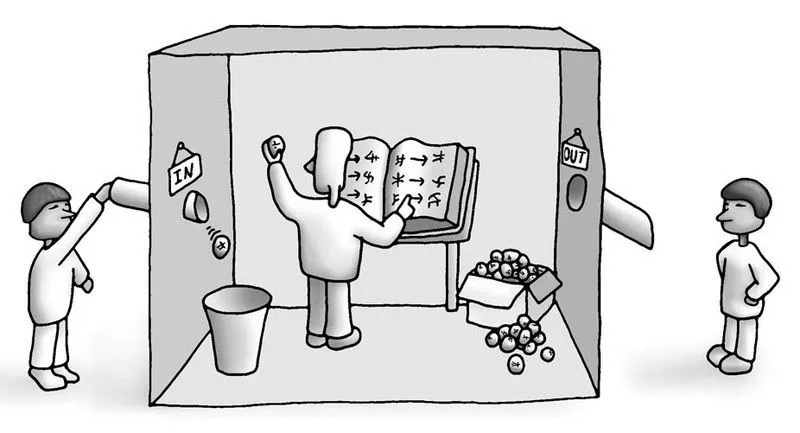
\includegraphics[width=0.8\textwidth]{o-quarto-chines.jpg}
% 			% \caption{Fonte: \citet{pinar2000turing}.}
% 		\end{figure}
% 	}
% 	\only<5>{
% 		Esse argumento evidencia a dificuldade presente em avaliar a real 
% 		capacidade de uma máquina executando tarefas humanas.
% 	}
% \end{frame}

%----------------------------------------------------------------------------------------

% \begin{frame}
% 	\frametitle{Large Language Models}
% \end{frame}

%----------------------------------------------------------------------------------------

\begin{frame}
	\frametitle{Open-Ended Tasks}
	\only<1-5>{
		\begin{itemize}[<+(1)->]
			\item Permitem diferentes interpretações e soluções. 
			\item Primariamente subjetivas.
			\item Comumente presente em áreas que exigem criatividade e pensamento crítico.
			\item Extremamente comuns em PLN.
		\end{itemize}
	}
	\only<6>{
		\frametitle{Exemplos}
		\begin{columns}
			\column{0.5\linewidth}
				\begin{figure}
					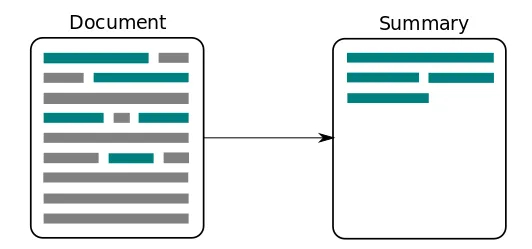
\includegraphics[width=0.8\textwidth]{summ.png}
					\caption{Sumarização}
				\end{figure}
			\column{0.5\linewidth}
				\begin{figure}
					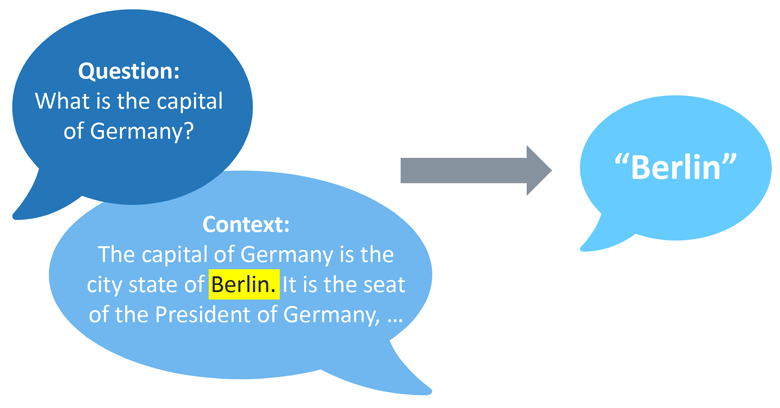
\includegraphics[width=0.8\textwidth]{qamainimage.png}
					\caption{Question-Answering}
				\end{figure}
		\end{columns}
	}
\end{frame}

%----------------------------------------------------------------------------------------

\begin{frame}
	\only<1>{
		\frametitle{Avaliação Intínseca x Extrínseca}
		\begin{figure}
			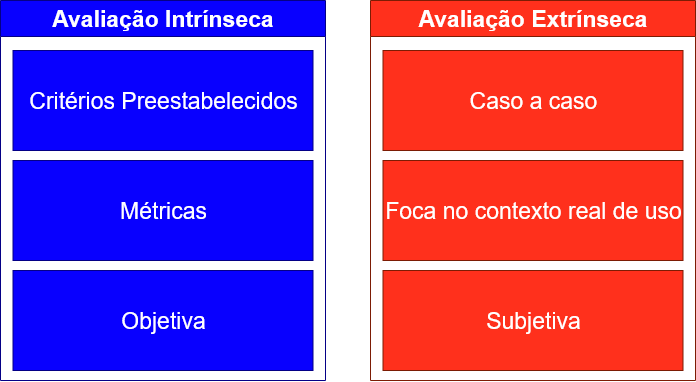
\includegraphics[width=0.8\textwidth]{TCC-Extrinsic-Intrinsic.png}
		\end{figure}
	}
	\only<3->{
		\frametitle{Avaliação de Open-Ended Tasks}
	}
	\only<2>{
		\frametitle{Avaliação Intínseca}
		\begin{figure}
			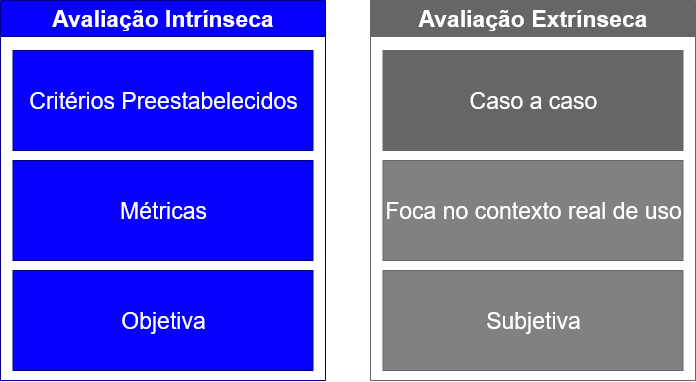
\includegraphics[width=0.8\textwidth]{TCC-Extrinsic-Intrinsic-Chosen.png}
		\end{figure}
	}
	\only<3>{
		\begin{figure}
			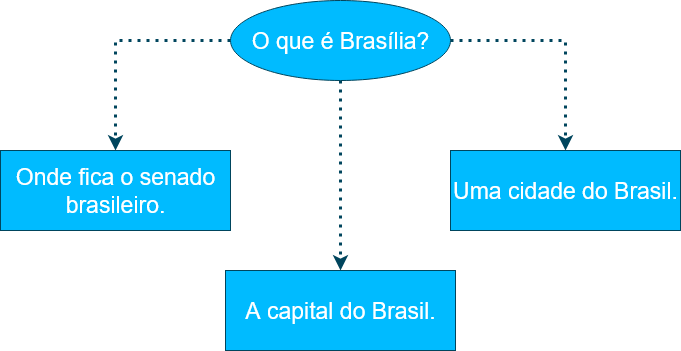
\includegraphics[width=0.8\textwidth]{TCC-qa-dificulty-example.png}
		\end{figure}
	}
	\only<4>{
		\begin{figure}
			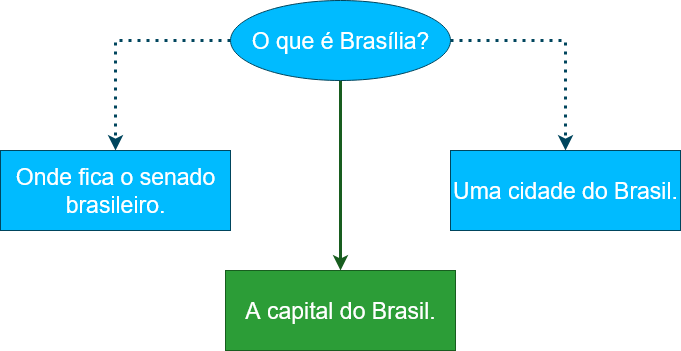
\includegraphics[width=0.8\textwidth]{TCC-qa-dificulty-example-resposta_esperada.png}
		\end{figure}
	}
	\only<5>{
		\begin{figure}
			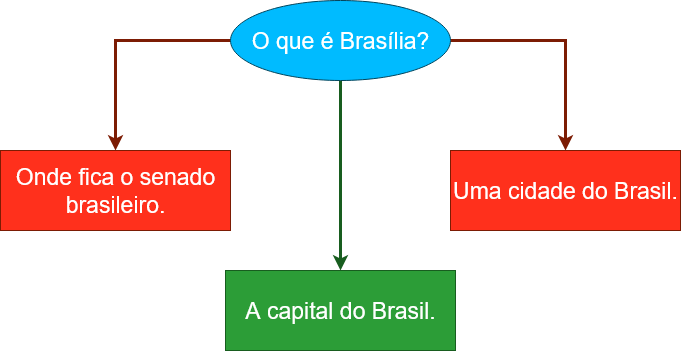
\includegraphics[width=0.8\textwidth]{TCC-qa-dificulty-example-problem.png}
		\end{figure}
	}
	\only<6>{
		\begin{figure}
			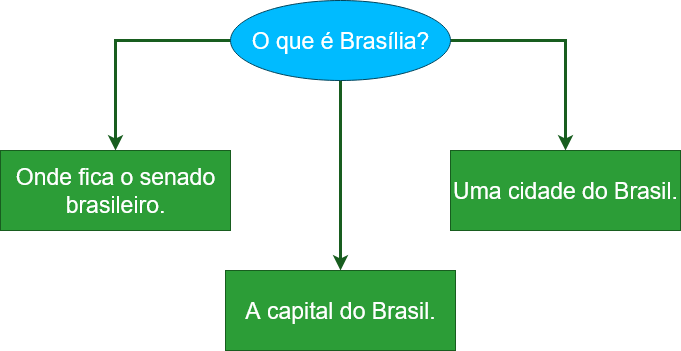
\includegraphics[width=0.8\textwidth]{TCC-qa-dificulty-example-esperado.png}
		\end{figure}
	}
	% \only<6->{
	% 	\begin{center}
	% 		Um cachorro foi ao parque se divertir, lá encontrou um gato. Após 
	% 		encontrá-lo o cachorro passou a tarde correndo atrás do mesmo.
	% 	\end{center}
	% 	\begin{columns}
	% 		\column{0.5\linewidth}
	% 		\begin{center}
	% 			O cachorro foi ao parque e brincou com o gato.
	% 		\end{center}
	% 		\column{0.5\linewidth}
	% 		\begin{center}
	% 			O cachorro passou a tarde correndo atrás do gato no parque.
	% 		\end{center}
	% 	\end{columns}
	% }
\end{frame}

%----------------------------------------------------------------------------------------

\begin{frame}
	\frametitle{Métricas Baseadas em N-Gramas}
	\only<2>{
		\begin{figure}
			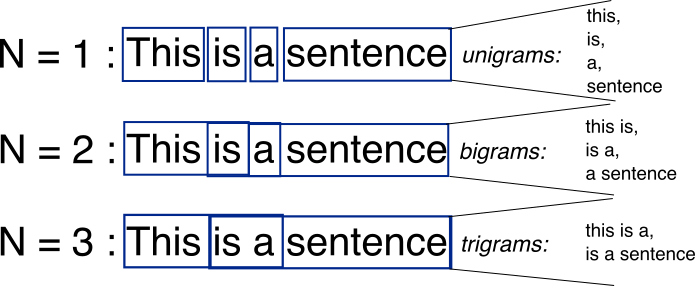
\includegraphics[width=0.8\textwidth]{n-grams.png}
		\end{figure}
	}
	\only<3>{
		\begin{figure}
			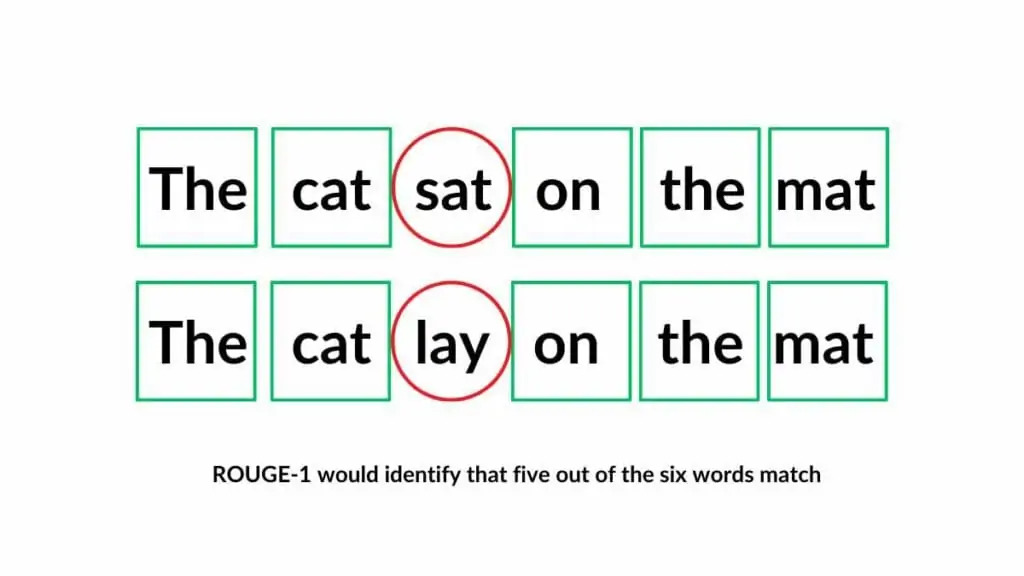
\includegraphics[width=0.8\textwidth]{ROUGE-1-example-1024x576.jpg}
		\end{figure}
	}
	\only<4>{
		\frametitle{Métricas Mais Populares}
		\begin{itemize}
			\item BLEU
			\item ROUGE
			\item METEOR
		\end{itemize}
	}
	\only<5-7>{
		\frametitle{Problemas desse tipo de métrica}
		\begin{itemize}[<+(5)->]
			\item Não capturam significado semântico.
			\item Dificuldade em reconhecer sinônimos.
		\end{itemize}
	}
	\only<8>{
		\frametitle{Problemas desse tipo de métrica}
		\begin{figure}
			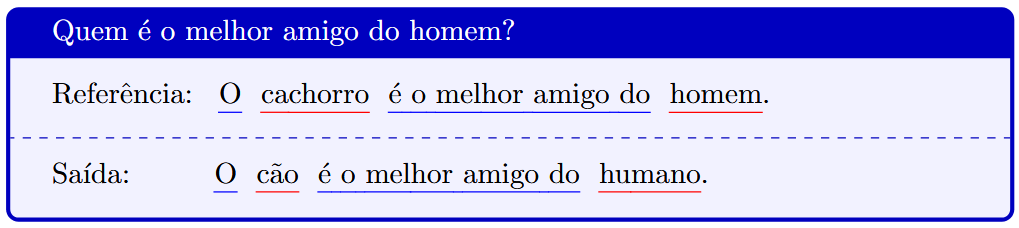
\includegraphics[width=0.9\textwidth]{sinonimos-problema.png}
		\end{figure}
	}
\end{frame}

%----------------------------------------------------------------------------------------

\begin{frame}
	\frametitle{Métricas Baseadas em PLMs}
	\only<2>{
		\begin{columns}
			\column{0.5\textwidth}
			\begin{figure}
				
\includegraphics[height=0.6\textheight]{Bert_smile.png}
				\caption{BERT (Devlin et al., 2019)}
			\end{figure}
			\column{0.5\textwidth}
			\begin{figure}
				
\includegraphics[height=0.6\textheight]{Simpsons_PNG93.png}
				\caption{BART (Lewis et al., 2019)}
			\end{figure}
		\end{columns}
	}
	\only<3>{
		\begin{figure}
			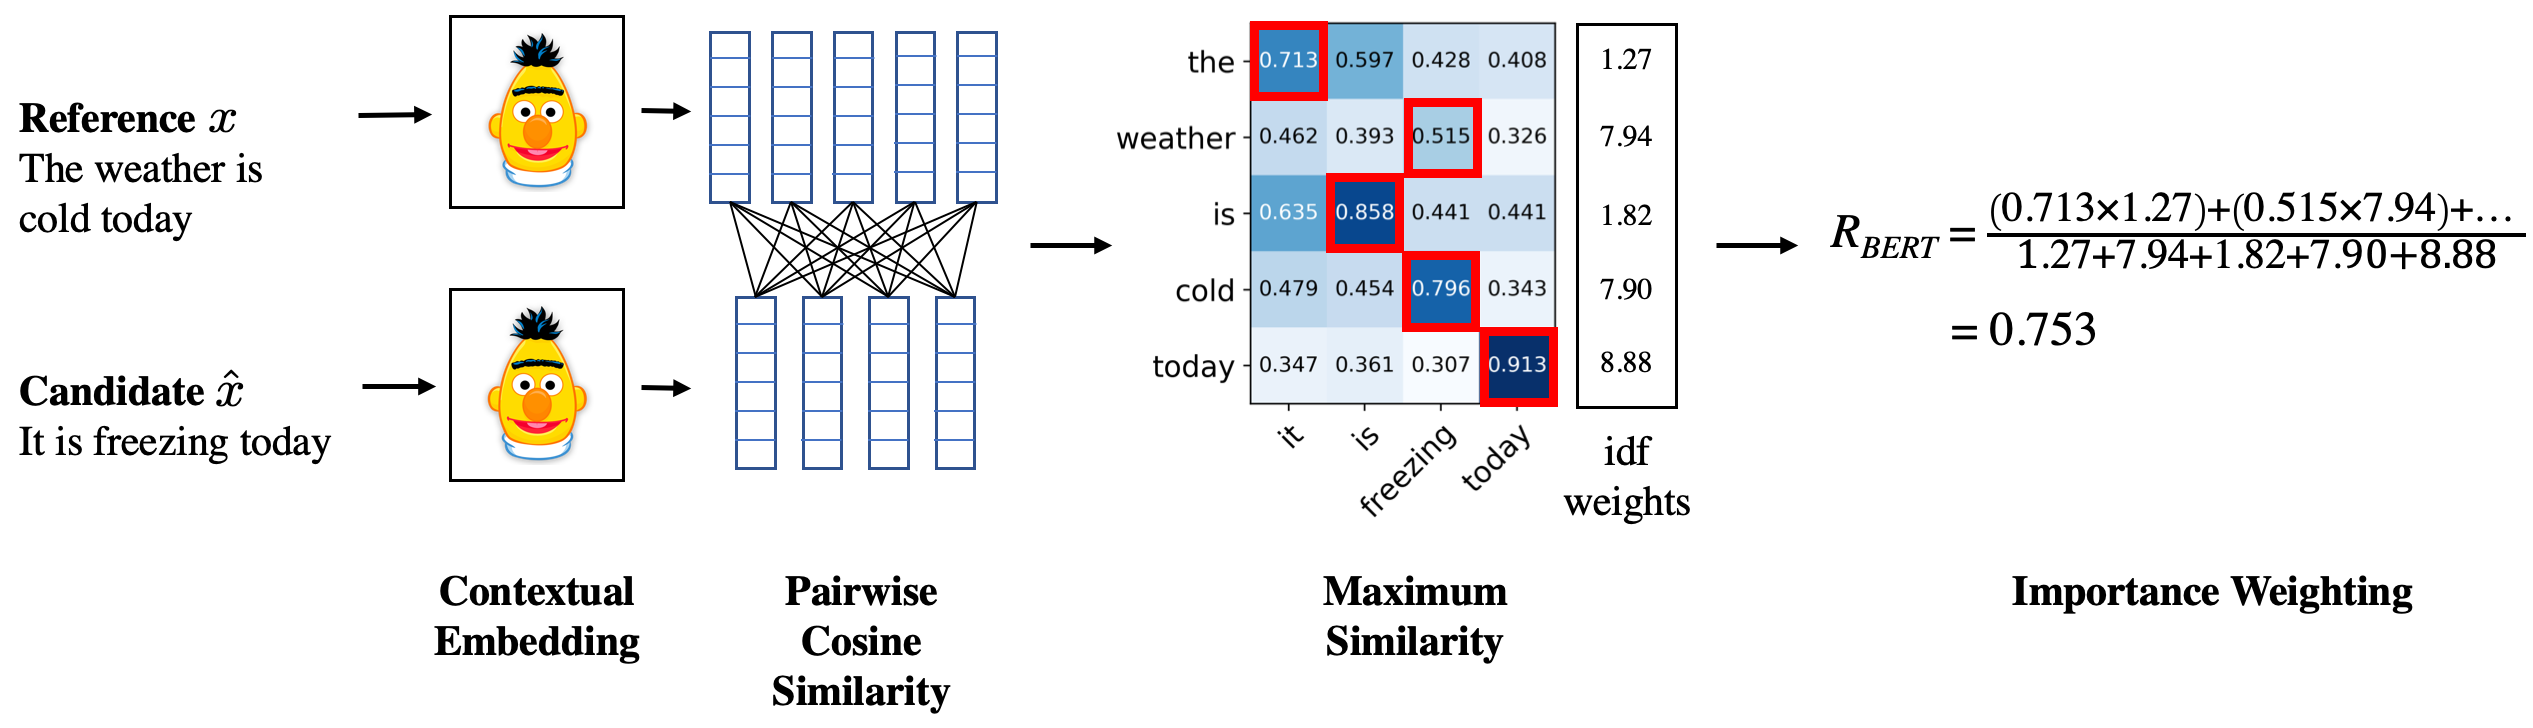
\includegraphics[width=\textwidth]{bert_score.png}
		\end{figure}
	}
	\only<4>{
		\frametitle{Métricas Mais Populares}
		\begin{itemize}
			\item BERTScore
			\item MoverScore
			\item BARTScore
		\end{itemize}
	}
	\only<5-8>{
		\frametitle{Problemas desse tipo de métrica}
		\begin{itemize}[<+(5)->]
			\item Alto custo computacional.
			\item Dependência de bons modelos.
			\item Caixa preta.
		\end{itemize}
	}
	\only<9>{
		\begin{figure}
			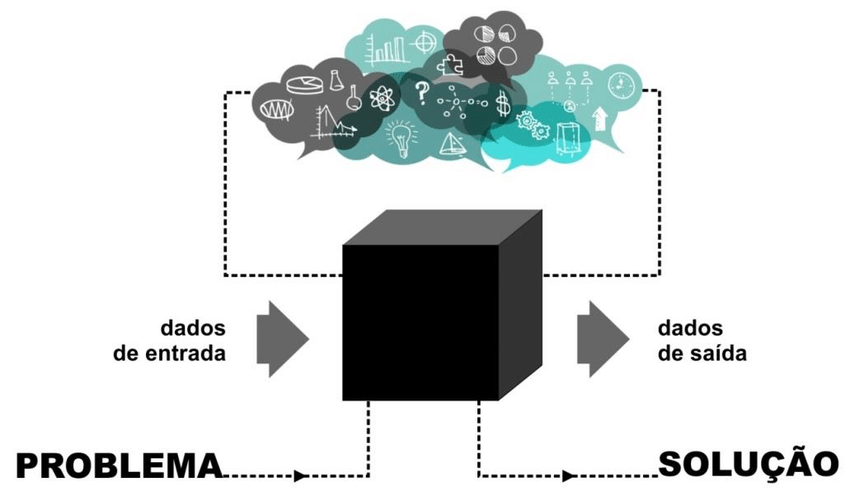
\includegraphics[width=0.9\textwidth]{Figura-31-Metodo-da-Caixa-Preta.png}
		\end{figure}
	}
\end{frame}

%----------------------------------------------------------------------------------------

\begin{frame}
	\frametitle{Problemática}
	\begin{itemize}[<+(1)->]
		\item Avaliar o desempenho de modelos é complexo.
		\item Novas métricas seguem surgindo.
		\item Qual métrica melhor se adequa a cada situação?
		\only<5>{
			\item Como as métricas se correlacionam com avaliação humana?
		}
		\only<6>{
			\item \textbf{Como as métricas se correlacionam com avaliação humana?}
		}
	\end{itemize}
\end{frame}

%----------------------------------------------------------------------------------------

\begin{frame}
	\frametitle{Objetivo}
	Mensurar a correlação entre diferentes métricas de avaliação automatizadas e 
	a forma de avaliação humana no âmbito de open-ended tasks.
\end{frame}